\documentclass{article}\usepackage[]{graphicx}\usepackage[]{color}
%% maxwidth is the original width if it is less than linewidth
%% otherwise use linewidth (to make sure the graphics do not exceed the margin)
\makeatletter
\def\maxwidth{ %
  \ifdim\Gin@nat@width>\linewidth
    \linewidth
  \else
    \Gin@nat@width
  \fi
}
\makeatother

\definecolor{fgcolor}{rgb}{0.345, 0.345, 0.345}
\newcommand{\hlnum}[1]{\textcolor[rgb]{0.686,0.059,0.569}{#1}}%
\newcommand{\hlstr}[1]{\textcolor[rgb]{0.192,0.494,0.8}{#1}}%
\newcommand{\hlcom}[1]{\textcolor[rgb]{0.678,0.584,0.686}{\textit{#1}}}%
\newcommand{\hlopt}[1]{\textcolor[rgb]{0,0,0}{#1}}%
\newcommand{\hlstd}[1]{\textcolor[rgb]{0.345,0.345,0.345}{#1}}%
\newcommand{\hlkwa}[1]{\textcolor[rgb]{0.161,0.373,0.58}{\textbf{#1}}}%
\newcommand{\hlkwb}[1]{\textcolor[rgb]{0.69,0.353,0.396}{#1}}%
\newcommand{\hlkwc}[1]{\textcolor[rgb]{0.333,0.667,0.333}{#1}}%
\newcommand{\hlkwd}[1]{\textcolor[rgb]{0.737,0.353,0.396}{\textbf{#1}}}%
\let\hlipl\hlkwb

\usepackage{framed}
\makeatletter
\newenvironment{kframe}{%
 \def\at@end@of@kframe{}%
 \ifinner\ifhmode%
  \def\at@end@of@kframe{\end{minipage}}%
  \begin{minipage}{\columnwidth}%
 \fi\fi%
 \def\FrameCommand##1{\hskip\@totalleftmargin \hskip-\fboxsep
 \colorbox{shadecolor}{##1}\hskip-\fboxsep
     % There is no \\@totalrightmargin, so:
     \hskip-\linewidth \hskip-\@totalleftmargin \hskip\columnwidth}%
 \MakeFramed {\advance\hsize-\width
   \@totalleftmargin\z@ \linewidth\hsize
   \@setminipage}}%
 {\par\unskip\endMakeFramed%
 \at@end@of@kframe}
\makeatother

\definecolor{shadecolor}{rgb}{.97, .97, .97}
\definecolor{messagecolor}{rgb}{0, 0, 0}
\definecolor{warningcolor}{rgb}{1, 0, 1}
\definecolor{errorcolor}{rgb}{1, 0, 0}
\newenvironment{knitrout}{}{} % an empty environment to be redefined in TeX

\usepackage{alltt}
\usepackage{natbib}
\usepackage[unicode=true]{hyperref}
\usepackage{geometry}
\usepackage{hyperref}
\usepackage{color}
\usepackage{amsmath}
\usepackage{amssymb}
\usepackage{verbatim}
\usepackage{mathpazo}
\usepackage{setspace}
\usepackage{multirow}
\usepackage{fullpage}
\usepackage{lscape}
\usepackage{fancyhdr}
\usepackage{wrapfig,lipsum,booktabs}
\usepackage[normalem]{ulem}
\usepackage[parfill]{parskip}
\usepackage{multirow}
\geometry{tmargin=1in,bmargin=1in,lmargin=1in,rmargin=1in}

\bibliographystyle{ecology_let}

%% for inline R code: if the inline code is not correctly parsed, you will see a message
\newcommand{\rinline}[1]{SOMETHING WRONG WITH knitr}


\IfFileExists{upquote.sty}{\usepackage{upquote}}{}
\begin{document}
\title{Proximity of restored hedgerows interacts with local floral diversity and species traits to shape  long-term pollinator metacommunity dynamics: a walk through of the models and analyses}
\author{Lauren Ponisio}


\maketitle

\begin{figure}[h!]
\centering
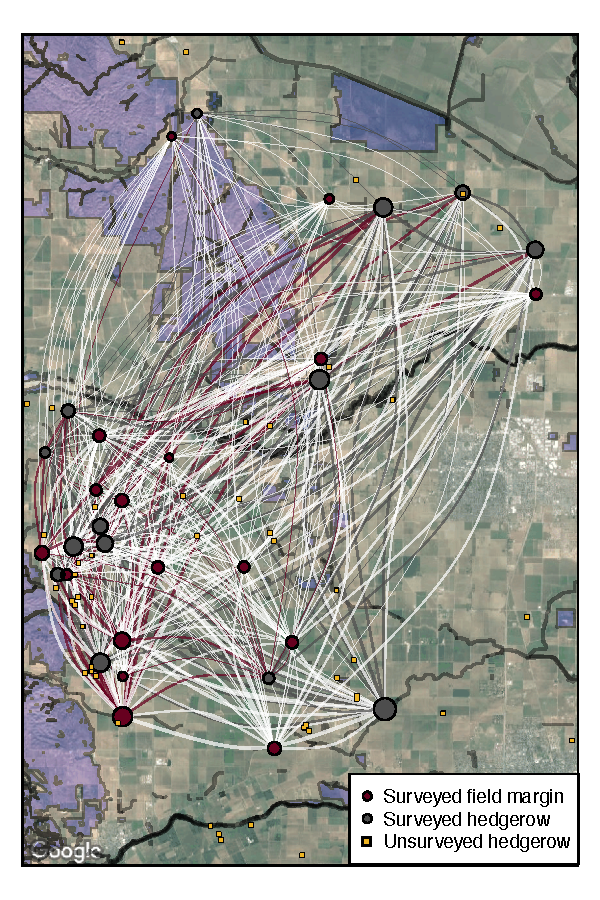
\includegraphics[width=0.6\textwidth]{figure/degree_spatial.pdf}
\label{fig:network}
\end{figure}
\clearpage

\section{Overview}
In our study we examine the metacommunity dynamics of plant-pollinator
communities using variety of different methods including 1) occupancy
modeling and 2) network analyses.  We are committed to reproducible
science and all analytical code will be maintained on github, along
with this write up.

The entire analysis is executable from the main.sh file. All of the
packages needed to run the analyses are listed in the packages.sh
file. All analyses were run using R (version $3.5.1$)
and nimble (0.6-12). 

Navigate to the analysis folder within the github repo
(hedgerow\_metacommunity) then the main.sh file can be selected and
run (a warning, the occupancy analyses each take several hours on my
2.3 GHz imac pro, so all together they will take quite a while), you
could run all of the analyses in the study by running this line in
BASH.

\begin{knitrout}
\definecolor{shadecolor}{rgb}{0.969, 0.969, 0.969}\color{fgcolor}\begin{kframe}
\begin{alltt}
bash main.sh
\end{alltt}
\end{kframe}
\end{knitrout}

This will somewhat helpfully print the results of each analysis
and re-create any accompanying figures.

We will walk through each the main script for each analysis
individually.

\section{Occupancy model}

The occupancy models are run through the main.R file in the
analysis/occupancy folder. The script begins by setting the arguments
for prepping the data. Run as is to reproduce the data used in the
study. Prior analyses used the area of hedgerows in buffers weighted
by log distance from a focal site instead of the Gaussian decay
method, with similar results. In addition, the method for calculating
the habitat quality of a patch can be toggled using the ``col.name.div.type" argument. Other options are plant richness
``Richness" or the diversity of flowers visited by pollinators
``div.visits". All measures gave qualitatively similar results.

Importantly, ``natural.decay" and ``HR.decay" change the decay
($\alpha$) of weighting of remnant and hedgerow area,
respectively. Different combinations ($350$, $1000$, and $2500$) can
be used to change the steepness of the decay rate from very steep
($\alpha=350$ represents $98.5\%$ reduction in weight by $1$ $km$) to
very shallow ($\alpha=2500$ represents a $98.5\%$ reduction in weight
by $7$ $km$). The main.sh script executes all combinations of decay
rates. They are executed individually because the nimble models take a
considerable amount of computer memory which is not cleared after the
model is run. Running them all in a four loop within the same instance
of R would overload most computers.

To run the MCMC in order to estimate the model coefficients, we use the
NIMBLE R package \citep{nimble-14, de2017programming}.  ``nimble"
stands for ``numerical inference for statistical models with Bayesian
and likelihood estimation."  It implements almost the same model
language as BUGS and JAGS, but supports easy customization of MCMC
algorithms, including writing new samplers, and user-defined functions
and distributions, which opens up enormous flexibility in how models
are written. This enabled us to integrate over the latent states,
increasing computational efficiency by an order of magnitude in
comparison to sampling every latent state. 


The multi-species, multi-season occupancy model is as follows (the
model code follows the notation in equation 5-6 in the manucript,
except $HRwtProx$ is abbreviated as $hr.area$, and $RemnantWtProx$ as
$nat.area$):


\begin{knitrout}
\definecolor{shadecolor}{rgb}{0.969, 0.969, 0.969}\color{fgcolor}\begin{kframe}
\begin{alltt}
\hlstd{ms.ms.occ}
\end{alltt}
\begin{verbatim}
## {
##     mu.p.0 ~ dnorm(0, 0.001)
##     mu.p.day.1 ~ dnorm(0, 0.001)
##     mu.p.day.2 ~ dnorm(0, 0.001)
##     sigma.p.0 ~ dunif(0, 100)
##     sigma.p.day.1 ~ dunif(0, 100)
##     sigma.p.day.2 ~ dunif(0, 100)
##     mu.phi.0 ~ dnorm(0, 0.001)
##     mu.gam.0 ~ dnorm(0, 0.001)
##     sigma.phi.0 ~ dunif(0, 100)
##     sigma.gam.0 ~ dunif(0, 100)
##     mu.phi.hr.area ~ dnorm(0, 0.001)
##     mu.gam.hr.area ~ dnorm(0, 0.001)
##     sigma.phi.hr.area ~ dunif(0, 100)
##     sigma.gam.hr.area ~ dunif(0, 100)
##     mu.phi.nat.area ~ dnorm(0, 0.001)
##     mu.gam.nat.area ~ dnorm(0, 0.001)
##     sigma.phi.nat.area ~ dunif(0, 100)
##     sigma.gam.nat.area ~ dunif(0, 100)
##     mu.phi.fra ~ dnorm(0, 0.001)
##     mu.gam.fra ~ dnorm(0, 0.001)
##     sigma.phi.fra ~ dunif(0, 100)
##     sigma.gam.fra ~ dunif(0, 100)
##     phi.k ~ dnorm(0, 0.001)
##     gam.k ~ dnorm(0, 0.001)
##     phi.B ~ dnorm(0, 0.001)
##     gam.B ~ dnorm(0, 0.001)
##     phi.hr.area.fra ~ dnorm(0, 0.001)
##     gam.hr.area.fra ~ dnorm(0, 0.001)
##     phi.nat.area.fra ~ dnorm(0, 0.001)
##     gam.nat.area.fra ~ dnorm(0, 0.001)
##     phi.hr.area.k ~ dnorm(0, 0.001)
##     gam.hr.area.k ~ dnorm(0, 0.001)
##     phi.nat.area.k ~ dnorm(0, 0.001)
##     gam.nat.area.k ~ dnorm(0, 0.001)
##     phi.hr.area.B ~ dnorm(0, 0.001)
##     gam.hr.area.B ~ dnorm(0, 0.001)
##     phi.nat.area.B ~ dnorm(0, 0.001)
##     gam.nat.area.B ~ dnorm(0, 0.001)
##     for (sp in 1:nsp) {
##         p.0[sp] ~ dnorm(mu.p.0, sd = sigma.p.0)
##         p.day.1[sp] ~ dnorm(mu.p.day.1, sd = sigma.p.day.1)
##         p.day.2[sp] ~ dnorm(mu.p.day.2, sd = sigma.p.day.2)
##         phi.0[sp] ~ dnorm(mu.phi.0, sd = sigma.phi.0)
##         gam.0[sp] ~ dnorm(mu.gam.0, sd = sigma.gam.0)
##         phi.hr.area[sp] ~ dnorm(mu.phi.hr.area, sd = sigma.phi.hr.area)
##         gam.hr.area[sp] ~ dnorm(mu.gam.hr.area, sd = sigma.gam.hr.area)
##         phi.nat.area[sp] ~ dnorm(mu.phi.nat.area, sd = sigma.phi.nat.area)
##         gam.nat.area[sp] ~ dnorm(mu.gam.nat.area, sd = sigma.gam.nat.area)
##         phi.fra[sp] ~ dnorm(mu.phi.fra, sd = sigma.phi.fra)
##         gam.fra[sp] ~ dnorm(mu.gam.fra, sd = sigma.gam.fra)
##     }
##     for (sp in 1:nsp) {
##         for (site in 1:nsite) {
##             for (yr in 1:nyear) {
##                 for (rep in 1:nrep[site, yr, sp]) {
##                   logit(p[site, yr, rep, sp]) <- p.0[sp] + p.day.1[sp] * 
##                     day[site, yr, rep, sp] + p.day.2[sp] * day.2[site, 
##                     yr, rep, sp]
##                 }
##             }
##             logit(phi.site.sp.mean[site, sp]) <- mean(phi[site, 
##                 1:(nyear - 1), sp])
##             logit(gam.site.sp.mean[site, sp]) <- mean(gam[site, 
##                 1:(nyear - 1), sp])
##             psi.1[site, sp] <- gam.site.sp.mean[site, sp]/(1 - 
##                 phi.site.sp.mean[site, sp] + gam.site.sp.mean[site, 
##                 sp])
##             psi[site, 1, sp] <- psi.1[site, sp]
##             for (yr in 1:(nyear - 1)) {
##                 phi[site, yr, sp] <- phi.0[sp] + phi.k * k[sp] + 
##                   phi.B * B[sp] + phi.hr.area[sp] * HRarea[site] + 
##                   phi.nat.area[sp] * natural[site] + phi.fra[sp] * 
##                   fra[site, yr] + phi.hr.area.fra * fra[site, 
##                   yr] * HRarea[site] + phi.nat.area.fra * fra[site, 
##                   yr] * natural[site] + phi.hr.area.k * k[sp] * 
##                   HRarea[site] + phi.nat.area.k * k[sp] * natural[site] + 
##                   phi.hr.area.B * B[sp] * HRarea[site] + phi.nat.area.B * 
##                   B[sp] * natural[site]
##                 gam[site, yr, sp] <- gam.0[sp] + gam.k * k[sp] + 
##                   gam.B * B[sp] + gam.hr.area[sp] * HRarea[site] + 
##                   gam.nat.area[sp] * natural[site] + gam.fra[sp] * 
##                   fra[site, yr] + gam.hr.area.fra * fra[site, 
##                   yr] * HRarea[site] + gam.nat.area.fra * fra[site, 
##                   yr] * natural[site] + gam.hr.area.k * k[sp] * 
##                   HRarea[site] + gam.nat.area.k * k[sp] * natural[site] + 
##                   gam.hr.area.B * B[sp] * HRarea[site] + gam.nat.area.B * 
##                   B[sp] * natural[site]
##             }
##         }
##     }
##     for (site in 1:nsite) {
##         for (sp in 1:nsp) {
##             X[site, 1:nyear, 1:max.nreps, sp] ~ dDynamicOccupancy(nrep = nrep[site, 
##                 1:nyear, sp], psi1 = psi[site, 1, sp], phi = expit(phi[site, 
##                 1:(nyear - 1), sp]), gamma = expit(gam[site, 
##                 1:(nyear - 1), sp]), p = p[site, 1:nyear, 1:max.nreps, 
##                 sp])
##         }
##     }
## }
\end{verbatim}
\end{kframe}
\end{knitrout}

For those of you familiar with working in BUGS or JAGS, the main
difference here is the call to 'dDynamicOccupancy'. This is the
function allows us to numerically integrate over sequences of latent
states to directly calculate model likelihoods, removing the need to
perform MCMC sampling of these latent variables.



\begin{knitrout}
\definecolor{shadecolor}{rgb}{0.969, 0.969, 0.969}\color{fgcolor}\begin{kframe}
\begin{alltt}
\hlstd{dDynamicOccupancy}
\end{alltt}
\begin{verbatim}
## function (x, nrep, psi1, phi, gamma, p, log = 0) 
## {
##     ProbOccNextTime <- psi1
##     ll <- 0
##     nyears <- nimDim(x)[1]
##     if (nyears >= 1) {
##         for (t in 1:nyears) {
##             if (nrep[t] > 0) {
##                 numObs <- sum(x[t, 1:nrep[t]])
##                 if (numObs < 0) {
##                   nimPrint("Error in dDynamicOccupancy: numObs < 0 but nrep[t] > 0\n")
##                   nimStop("Error in dDynamicOccupancy: numObs < 0 but nrep[t] > 0\n")
##                 }
##                 ProbOccAndCount <- ProbOccNextTime * exp(sum(dbinom(x[t, 
##                   1:nrep[t]], size = 1, p = p[t, 1:nrep[t]], 
##                   log = 1)))
##                 ProbUnoccAndCount <- (1 - ProbOccNextTime) * 
##                   (numObs == 0)
##                 ProbCount <- ProbOccAndCount + ProbUnoccAndCount
##                 ProbOccGivenCount <- ProbOccAndCount/ProbCount
##                 ll <- ll + log(ProbCount)
##                 if (t < nyears) 
##                   ProbOccNextTime <- ProbOccGivenCount * phi[t] + 
##                     (1 - ProbOccGivenCount) * gamma[t]
##             }
##             else {
##                 if (t < nyears) 
##                   ProbOccNextTime <- ProbOccNextTime * phi[t] + 
##                     (1 - ProbOccNextTime) * gamma[t]
##             }
##         }
##     }
##     if (log) 
##         return(ll)
##     else return(exp(ll))
## }
## <environment: 0x7f88f4c125f8>
\end{verbatim}
\end{kframe}
\end{knitrout}

The number of MCMC iterations, burnin, number of chains, etc. can be
toggled by changing the value of the scale object. This script will
also generate MCMC diagnostic figures ($src\_plotting/checkChains.R$),
interaction plots ($src\_plotting/plotInteractions.R$), and posterior
mean and credible internal plots and table ($src\_plotting/posteriorPlotting.R$).


\section{Metacommunity Network Analysis}

The 'spTempMets.R' file executes the network analyses. The  user can
provide any network metrics taken by the function 'speciesLevel' in
the bipartite package. The  $y_{i,j,k}$ network
metrics of the $i^{\mathrm{th}}$ species at the $j^{\mathrm{th}}$ site
in the $k^{\mathrm{th}}$ year was modeled as:

%
\begin{equation}
\label{eq:lms}
\begin{split}
\mathrm{y}_{i,j,k} \sim \mathrm{B}_{i} + \mathrm{k}_{i} +
\mathrm{site}_{j} + \mathrm{site}_{k} \\   
\mathrm{site}_{j} \sim N(0, \sigma_{site}) \\  
\mathrm{year}_{k} \sim N(0, \sigma_{year})
\hspace{0.2em}
\end{split}
\end{equation}
%





The results for how species traits affect the role of pollinators in
the spatial metacommmunity network: 
\begin{knitrout}
\definecolor{shadecolor}{rgb}{0.969, 0.969, 0.969}\color{fgcolor}\begin{kframe}
\begin{alltt}
\hlkwd{lapply}\hlstd{(mod.years.pol, summary)}
\end{alltt}
\begin{verbatim}
## $k
## Linear mixed model fit by REML. t-tests use Satterthwaite's method [
## lmerModLmerTest]
## Formula: x
##    Data: specs.years.pol
## 
## REML criterion at convergence: 557
## 
## Scaled residuals: 
##     Min      1Q  Median      3Q     Max 
## -3.0281 -0.4275 -0.0558  0.3588  3.4899 
## 
## Random effects:
##  Groups       Name        Variance Std.Dev.
##  GenusSpecies (Intercept) 0.09441  0.3073  
##  Site         (Intercept) 0.01585  0.1259  
##  Residual                 0.16260  0.4032  
## Number of obs: 413, groups:  GenusSpecies, 102; Site, 10
## 
## Fixed effects:
##              Estimate Std. Error        df t value Pr(>|t|)    
## (Intercept)  -0.05166    0.05682  20.54598  -0.909   0.3738    
## r.degree      0.75945    0.04553  92.12789  16.680   <2e-16 ***
## MeanITD      -0.09329    0.04015 115.53534  -2.324   0.0219 *  
## ---
## Signif. codes:  0 '***' 0.001 '**' 0.01 '*' 0.05 '.' 0.1 ' ' 1
## 
## Correlation of Fixed Effects:
##          (Intr) r.degr
## r.degree 0.169        
## MeanITD  0.008  0.144 
## 
## $weighted.betweenness
## Linear mixed model fit by REML. t-tests use Satterthwaite's method [
## lmerModLmerTest]
## Formula: x
##    Data: specs.years.pol
## 
## REML criterion at convergence: -1017.5
## 
## Scaled residuals: 
##     Min      1Q  Median      3Q     Max 
## -6.7043 -0.1604 -0.0414  0.1147  7.8436 
## 
## Random effects:
##  Groups       Name        Variance Std.Dev.
##  GenusSpecies (Intercept) 0.00151  0.03886 
##  Site         (Intercept) 0.00000  0.00000 
##  Residual                 0.00381  0.06173 
## Number of obs: 413, groups:  GenusSpecies, 102; Site, 10
## 
## Fixed effects:
##               Estimate Std. Error         df t value Pr(>|t|)    
## (Intercept)   0.025858   0.005359 110.137374   4.825 4.53e-06 ***
## r.degree      0.057224   0.006035  95.986259   9.481 1.94e-15 ***
## MeanITD      -0.005847   0.005419 124.159779  -1.079    0.283    
## ---
## Signif. codes:  0 '***' 0.001 '**' 0.01 '*' 0.05 '.' 0.1 ' ' 1
## 
## Correlation of Fixed Effects:
##          (Intr) r.degr
## r.degree 0.217        
## MeanITD  0.014  0.150
\end{verbatim}
\end{kframe}
\end{knitrout}


And for how species traits affect the role of pollinators in
the temporal metacommmunity network: 
\begin{knitrout}
\definecolor{shadecolor}{rgb}{0.969, 0.969, 0.969}\color{fgcolor}\begin{kframe}
\begin{alltt}
\hlkwd{lapply}\hlstd{(mod.sites.pol, summary)}
\end{alltt}
\begin{verbatim}
## $k
## Linear mixed model fit by REML. t-tests use Satterthwaite's method [
## lmerModLmerTest]
## Formula: x
##    Data: specs.site.pol
## 
## REML criterion at convergence: 839
## 
## Scaled residuals: 
##     Min      1Q  Median      3Q     Max 
## -3.1765 -0.5764 -0.1379  0.3329  4.0470 
## 
## Random effects:
##  Groups       Name        Variance Std.Dev.
##  GenusSpecies (Intercept) 0.036829 0.19191 
##  Site         (Intercept) 0.008274 0.09096 
##  Residual                 0.368523 0.60706 
## Number of obs: 429, groups:  GenusSpecies, 98; Site, 17
## 
## Fixed effects:
##             Estimate Std. Error       df t value Pr(>|t|)    
## (Intercept) -0.03852    0.04514 21.74320  -0.853    0.403    
## r.degree     0.71464    0.04454 46.96095  16.046   <2e-16 ***
## MeanITD     -0.05535    0.03911 97.36820  -1.415    0.160    
## ---
## Signif. codes:  0 '***' 0.001 '**' 0.01 '*' 0.05 '.' 0.1 ' ' 1
## 
## Correlation of Fixed Effects:
##          (Intr) r.degr
## r.degree  0.136       
## MeanITD  -0.022  0.221
## 
## $weighted.betweenness
## Linear mixed model fit by REML. t-tests use Satterthwaite's method [
## lmerModLmerTest]
## Formula: x
##    Data: specs.site.pol
## 
## REML criterion at convergence: -601.4
## 
## Scaled residuals: 
##     Min      1Q  Median      3Q     Max 
## -3.1409 -0.2313 -0.0816  0.1394  6.5257 
## 
## Random effects:
##  Groups       Name        Variance Std.Dev.
##  GenusSpecies (Intercept) 0.001316 0.03628 
##  Site         (Intercept) 0.000000 0.00000 
##  Residual                 0.012708 0.11273 
## Number of obs: 429, groups:  GenusSpecies, 98; Site, 17
## 
## Fixed effects:
##               Estimate Std. Error         df t value Pr(>|t|)    
## (Intercept)   0.038922   0.007243  97.667693   5.374 5.24e-07 ***
## r.degree      0.075158   0.008329  71.313326   9.024 2.04e-13 ***
## MeanITD      -0.007204   0.007262 137.218365  -0.992    0.323    
## ---
## Signif. codes:  0 '***' 0.001 '**' 0.01 '*' 0.05 '.' 0.1 ' ' 1
## 
## Correlation of Fixed Effects:
##          (Intr) r.degr
## r.degree  0.173       
## MeanITD  -0.035  0.222
\end{verbatim}
\end{kframe}
\end{knitrout}


Lastly, for how patch ``traits" affect their role in spatial  metacommmunity network: 
\begin{knitrout}
\definecolor{shadecolor}{rgb}{0.969, 0.969, 0.969}\color{fgcolor}\begin{kframe}
\begin{alltt}
\hlkwd{lapply}\hlstd{(mod.years.site, summary)}
\end{alltt}
\begin{verbatim}
## $k
## Linear mixed model fit by REML. t-tests use Satterthwaite's method [
## lmerModLmerTest]
## Formula: x
##    Data: specs.years.site
## 
## REML criterion at convergence: 398.3
## 
## Scaled residuals: 
##     Min      1Q  Median      3Q     Max 
## -1.8047 -0.6924 -0.1022  0.5191  2.7629 
## 
## Random effects:
##  Groups       Name        Variance Std.Dev.
##  GenusSpecies (Intercept) 0.3167   0.5627  
##  Site         (Intercept) 0.0000   0.0000  
##  Residual                 0.4947   0.7033  
## Number of obs: 163, groups:  GenusSpecies, 31; Site, 10
## 
## Fixed effects:
##              Estimate Std. Error        df t value Pr(>|t|)    
## (Intercept)   0.01499    0.11809  25.22235   0.127    0.900    
## Div           0.28437    0.06903 157.27042   4.120 6.12e-05 ***
## natArea      -0.02375    0.10887  28.87677  -0.218    0.829    
## hrArea        0.16699    0.13577  21.48215   1.230    0.232    
## ---
## Signif. codes:  0 '***' 0.001 '**' 0.01 '*' 0.05 '.' 0.1 ' ' 1
## 
## Correlation of Fixed Effects:
##         (Intr) Div    natAre
## Div      0.011              
## natArea -0.060 -0.059       
## hrArea   0.069  0.050  0.167
## 
## $weighted.betweenness
## Linear mixed model fit by REML. t-tests use Satterthwaite's method [
## lmerModLmerTest]
## Formula: x
##    Data: specs.years.site
## 
## REML criterion at convergence: -190.5
## 
## Scaled residuals: 
##     Min      1Q  Median      3Q     Max 
## -1.6527 -0.3194 -0.1939 -0.0430  6.1733 
## 
## Random effects:
##  Groups       Name        Variance Std.Dev.
##  GenusSpecies (Intercept) 0.003197 0.05655 
##  Site         (Intercept) 0.000000 0.00000 
##  Residual                 0.013625 0.11673 
## Number of obs: 163, groups:  GenusSpecies, 31; Site, 10
## 
## Fixed effects:
##               Estimate Std. Error         df t value Pr(>|t|)   
## (Intercept)   0.048898   0.014083  29.699705   3.472  0.00161 **
## Div           0.023152   0.010796 154.423397   2.145  0.03355 * 
## natArea      -0.002564   0.013378  37.990886  -0.192  0.84902   
## hrArea        0.029587   0.015608  22.753103   1.896  0.07079 . 
## ---
## Signif. codes:  0 '***' 0.001 '**' 0.01 '*' 0.05 '.' 0.1 ' ' 1
## 
## Correlation of Fixed Effects:
##         (Intr) Div    natAre
## Div      0.015              
## natArea -0.046 -0.090       
## hrArea   0.051  0.076  0.148
\end{verbatim}
\end{kframe}
\end{knitrout}


The plotting is then executed in the accompanying
$plotting/spTempMets.R$ script.

\clearpage

\begin{figure} \centering
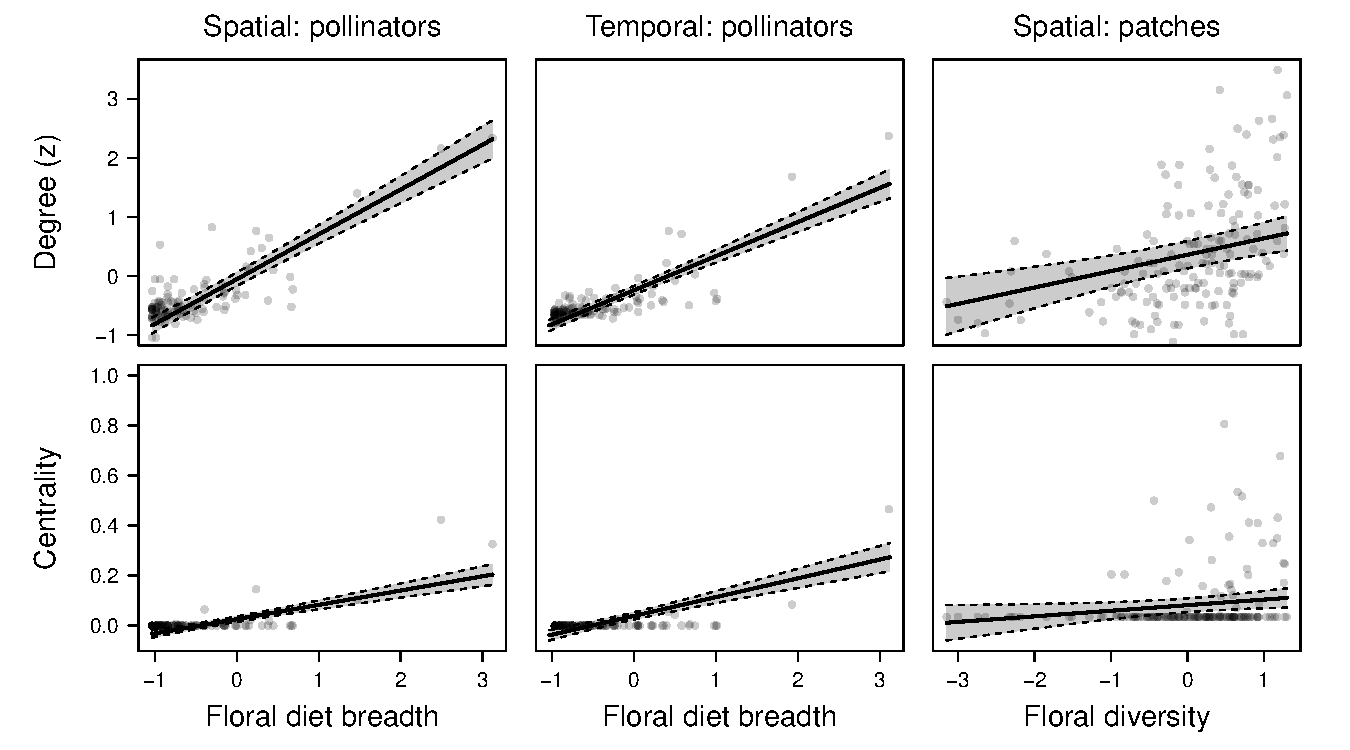
\includegraphics[width=1\textwidth]{figure/all_sig_drop_li_htFALSE.pdf}
\label{fig:connectivity} \caption{The relationship between species and
patch traits and their position in the metacommunity network when the
supergeneralists are not included in the community. Floral diet
breadth was positively related to both species degree (standardized)
and centrality and floral within a year across patches (spatial
network) and within a patch across years (temporal network). Body size
(mean intertegular distance, mm) was negatively related to species
degree but not centrality in the spatial network.  In addition, the
floral diversity of a patch was positively related to its degree and
centrality (marginally significant) within the patch network within a
year. Points represent means for each species or patch. The solid line
indicates the mean slope estimate and the dashed lines are the $95\%$
confidence intervals around the estimate.}  \end{figure} \clearpage






The results for how species traits affect the role of pollinators in
the spatial metacommmunity network without supergeneralists: 
\begin{knitrout}
\definecolor{shadecolor}{rgb}{0.969, 0.969, 0.969}\color{fgcolor}\begin{kframe}
\begin{alltt}
\hlkwd{lapply}\hlstd{(mod.years.pol, summary)}
\end{alltt}
\begin{verbatim}
## $k
## Linear mixed model fit by REML. t-tests use Satterthwaite's method [
## lmerModLmerTest]
## Formula: x
##    Data: specs.years.pol
## 
## REML criterion at convergence: 767.9
## 
## Scaled residuals: 
##     Min      1Q  Median      3Q     Max 
## -3.3223 -0.4184 -0.0923  0.3166  3.7501 
## 
## Random effects:
##  Groups       Name        Variance Std.Dev.
##  GenusSpecies (Intercept) 0.1755   0.41892 
##  Site         (Intercept) 0.0093   0.09644 
##  Residual                 0.3026   0.55012 
## Number of obs: 393, groups:  GenusSpecies, 100; Site, 10
## 
## Fixed effects:
##              Estimate Std. Error        df t value Pr(>|t|)    
## (Intercept)  -0.06969    0.06361  34.03898  -1.096   0.2810    
## r.degree      0.56697    0.05783 104.66451   9.804   <2e-16 ***
## MeanITD      -0.11872    0.05480 117.17997  -2.167   0.0323 *  
## ---
## Signif. codes:  0 '***' 0.001 '**' 0.01 '*' 0.05 '.' 0.1 ' ' 1
## 
## Correlation of Fixed Effects:
##          (Intr) r.degr
## r.degree 0.214        
## MeanITD  0.003  0.012 
## 
## $weighted.betweenness
## Linear mixed model fit by REML. t-tests use Satterthwaite's method [
## lmerModLmerTest]
## Formula: x
##    Data: specs.years.pol
## 
## REML criterion at convergence: -1183.1
## 
## Scaled residuals: 
##     Min      1Q  Median      3Q     Max 
## -3.6166 -0.1857 -0.0309  0.0624  7.3648 
## 
## Random effects:
##  Groups       Name        Variance Std.Dev.
##  GenusSpecies (Intercept) 0.002304 0.04800 
##  Site         (Intercept) 0.000000 0.00000 
##  Residual                 0.001805 0.04249 
## Number of obs: 393, groups:  GenusSpecies, 100; Site, 10
## 
## Fixed effects:
##               Estimate Std. Error         df t value Pr(>|t|)    
## (Intercept)   0.023876   0.005808 106.531229   4.111 7.78e-05 ***
## r.degree      0.035537   0.006057 108.007658   5.867 4.93e-08 ***
## MeanITD      -0.005655   0.005648 118.283865  -1.001    0.319    
## ---
## Signif. codes:  0 '***' 0.001 '**' 0.01 '*' 0.05 '.' 0.1 ' ' 1
## 
## Correlation of Fixed Effects:
##          (Intr) r.degr
## r.degree 0.326        
## MeanITD  0.004  0.002
\end{verbatim}
\end{kframe}
\end{knitrout}


And for how species traits affect the role of pollinators in
the temporal metacommmunity network without super generalists: 
\begin{knitrout}
\definecolor{shadecolor}{rgb}{0.969, 0.969, 0.969}\color{fgcolor}\begin{kframe}
\begin{alltt}
\hlkwd{lapply}\hlstd{(mod.sites.pol, summary)}
\end{alltt}
\begin{verbatim}
## $k
## Linear mixed model fit by REML. t-tests use Satterthwaite's method [
## lmerModLmerTest]
## Formula: x
##    Data: specs.site.pol
## 
## REML criterion at convergence: 919.9
## 
## Scaled residuals: 
##     Min      1Q  Median      3Q     Max 
## -3.1393 -0.5599 -0.1581  0.2961  3.4808 
## 
## Random effects:
##  Groups       Name        Variance Std.Dev.
##  GenusSpecies (Intercept) 0.06921  0.2631  
##  Site         (Intercept) 0.00000  0.0000  
##  Residual                 0.62262  0.7891  
## Number of obs: 372, groups:  GenusSpecies, 95; Site, 15
## 
## Fixed effects:
##              Estimate Std. Error        df t value Pr(>|t|)    
## (Intercept)  -0.02572    0.05326  81.36366  -0.483    0.631    
## r.degree      0.48541    0.05630  73.50603   8.623 9.04e-13 ***
## MeanITD      -0.06897    0.05278 100.38555  -1.307    0.194    
## ---
## Signif. codes:  0 '***' 0.001 '**' 0.01 '*' 0.05 '.' 0.1 ' ' 1
## 
## Correlation of Fixed Effects:
##          (Intr) r.degr
## r.degree  0.141       
## MeanITD  -0.034  0.059
## 
## $weighted.betweenness
## Linear mixed model fit by REML. t-tests use Satterthwaite's method [
## lmerModLmerTest]
## Formula: x
##    Data: specs.site.pol
## 
## REML criterion at convergence: -496.9
## 
## Scaled residuals: 
##     Min      1Q  Median      3Q     Max 
## -2.6593 -0.3989 -0.1419  0.0920  6.6031 
## 
## Random effects:
##  Groups       Name        Variance Std.Dev.
##  GenusSpecies (Intercept) 0.001649 0.0406  
##  Site         (Intercept) 0.000000 0.0000  
##  Residual                 0.013291 0.1153  
## Number of obs: 372, groups:  GenusSpecies, 95; Site, 15
## 
## Fixed effects:
##               Estimate Std. Error         df t value Pr(>|t|)    
## (Intercept)   0.036438   0.007956  99.335554   4.580 1.35e-05 ***
## r.degree      0.045370   0.008419  91.554906   5.389 5.47e-07 ***
## MeanITD      -0.012505   0.007865 122.245992  -1.590    0.114    
## ---
## Signif. codes:  0 '***' 0.001 '**' 0.01 '*' 0.05 '.' 0.1 ' ' 1
## 
## Correlation of Fixed Effects:
##          (Intr) r.degr
## r.degree  0.154       
## MeanITD  -0.036  0.057
\end{verbatim}
\end{kframe}
\end{knitrout}
\clearpage


\begin{figure} \centering
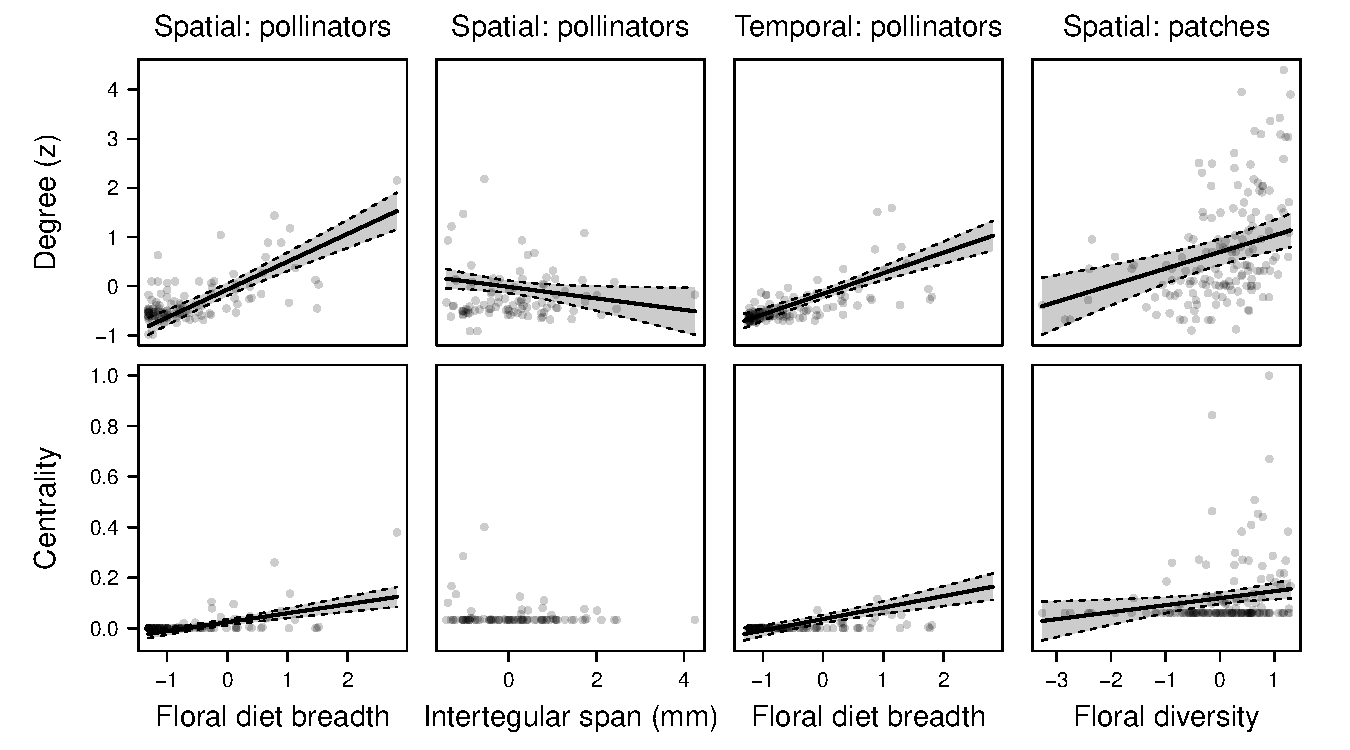
\includegraphics[width=1\textwidth]{figure/all_sig_drop_li_htTRUE.pdf}
\label{fig:connectivity} \caption{The relationship between species and
patch traits and their position in the metacommunity network when the
supergeneralists are not included in the community. Floral diet
breadth was positively related to both species degree (standardized)
and centrality and floral within a year across patches (spatial
network) and within a patch across years (temporal network). Body size
(mean intertegular distance, mm) was negatively related to species
degree but not centrality in the spatial network.  In addition, the
floral diversity of a patch was positively related to its degree and
centrality (marginally significant) within the patch network within a
year. Points represent means for each species or patch. The solid line
indicates the mean slope estimate and the dashed lines are the $95\%$
confidence intervals around the estimate.}  \end{figure} \clearpage


\clearpage
\bibliography{refs}
\clearpage


\end{document}
